%ltex: language=de-de
\chapter{Detaillierung}
	Die Transporteinheit \textit{nICE.cube} erfüllt den Zweck, Krisengebiete mit extremen Wetterbedingungen mit Medikamente und Impfstoffe zu versorgen, indem das Kühlgut
	sicher transportiert werden kann.\\
	Die Kühlung des Nutzvolumens erfolgt durch eine Kompressionskälteanlage mit einer maximalen Kühlleistung von \SI{27,65}{W}. Die zentrale Komponente bildet hier ein
	Kompressor der \textit{CASCADE}-Serie des Herstellers \textit{Masterflux} -- ein in seiner Klasse besonders energieeffizientes und spezifisch für den Einsatz im
	medizinischen Sektor entwickeltes Gerät.
	
	Die hervorragende thermische Isolation des Primärvolumens durch Graphen-Aerogel (vgl. \cref{tab:isomaterial}) reduziert die Betriebszeiten der Kälteanlage und damit den
	Energiebedarf des \textit{nICE.cube} auf ein Minimum.

	Zum autarken Betrieb ist ein Energiespeicher bestehend aus 32 Li-Ion-Zellen der Bauform 18650 verbaut. In 4S8P-Konfiguration liefern sie eine nominelle Versorgungsspannung
	der Systemkomponenten von \SI{14,8}{\volt} bei einer Gesamtkapazität von \SI{296}{\watt\hour} \footnote{Reduktion durch Verschleiß/Nutzungsverhalten möglich.}. Die bereits geringe
	Belastung des Energiespeichers durch Entladeströme je Zelle bei Volllast von \(\approx \SI{0,25}{A}\) wird durch thermische Überwachung jeder Einzelzelle garantiert. Über die Lebensdauer
	hinweg werden Lade- und Entladezyklen sowie Ströme und Spannungsverläufe aufgezeichnet, um die Nutzenden jederzeit über den Zustand des Akkus informieren zu können.
	
	Die Ladung erfolgt wahlweise stationär durch das lokale AC-Versorgungsnetz oder im mobilen Einsatz durch Anschluss eines Photovoltaikmoduls.
	Die äußeren Dimensionen des \textit{nICE.cube} betragen \( \SI{(813 \times 358 \times 314)}{mm} \) (LxBxH). Als Nutzvolumen steht mit Abmessungen von \( \approx \SI{(400 \times 248 \times 173) }{mm} \)
	ein Volumen von $ \SI{16,72}{L} $ zur Verfügung.

	\begin{figure}[h]
		\centering
		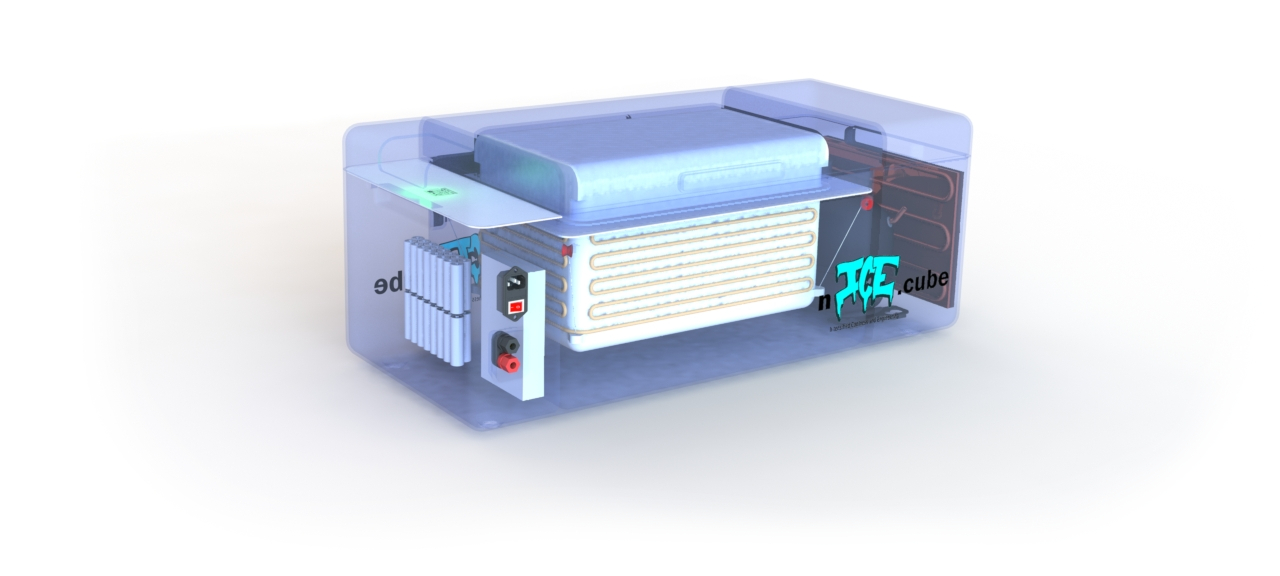
\includegraphics[width=\textwidth]{assets/transp6_edit.JPG}
		\caption[Konzeptansicht des \textit{nICE.cube}]{Konzeptansicht des \textit{nICE.cube} mit Blick auf die innenliegenden Komponenten.}
		\label{fig:transparent render}
	\end{figure}
	\clearpage
	\section{Stückliste}
		\begin{table}[h]
			\centering
			\caption{Stückliste (vgl. \cref{fig:explo})}
			\begin{tabular}[c]{@{}p{.05\textwidth}p{.06\textwidth}p{.07\textwidth}p{.35\textwidth}p{.35\textwidth}@{}}
				\toprule
				Pos. & Menge & Einheit & Benennung & Bemerkung\\
				\midrule
				1&1&Stk.&Ansaugverbindung& \\
				2&4&Stk.&Aramidschnur& \\
				3&1&Stk.&Druckreduzierer& \\
				4&2&Stk.&Durchführung&\\
				5&1&Stk.&Dämpfer&\\
				6&1&Stk.&E-Ink Display&1.54"\\
				7&1&Stk.&Ein-/Ausgabepanel& \\
				8&4&Stk.&Elektronik& \\
				9&1&Stk.&Elektronikdeckel& \\
				10&1&Stk.&Gummimanschette& \\
				11&1&Stk.&Hülle&\\
				12&1&Stk.&Kompressor&\textit{CASCADE17-0146Y1}\\
				13&1&Stk.&Kompressordeckel& \\
				14&1&Stk.&Kältemittelverbindung von\newline Verflüssiger& \\
				15&1&Stk.&Kältemittelverbindung zu\newline Verflüssiger& \\
				16&32&Stk.&Li-Ion 18650&4S8P Konfiguration\\
				17&1&Stk.&Reduzierer& \\
				18&1&Stk.&Transportgutbehälter&\\
				19&1&Stk.&Trockner&\\
				20&1&Stk.&Verflüssiger&\\
				21&1&Stk.&Verschlussdeckel außen&\\
				22&1&Stk.&Verschlussdeckel innen&\\
				23&1&Stk.&DC-Anschluss&Buchse für \SI{4,2}{mm} Laborstecker mit Polschraube (Bipolar)\\
				24&1&Stk.&AC-Anschluss&C14 AC Buchse mit Schalter und Sicherungshalter\\
				\bottomrule
			\end{tabular}
			\label{tab:stueckliste}
		\end{table}